This chapter provides an introduction to the thesis.
We first discuss the importance of mathematical models,
and then introduce rhythmic phenomena and coupled phase-oscillator models, which are the central topics of this thesis.
Finally, the outline of this thesis is summarized.

\section{Mathematical modeling}

% Humans have always been challenged to discover the principles behind complex natural phenomena and to predict the future from them. Astronomical observations were developed by the ancient Greeks because the solar calendar was very important for their agricultural activities, and in the last few years there has been an increasing need to create predictive models of the number of people infected in order to combat new coronaviruses. Perhaps the most important equation among these examples is the equation of motion, which describes the motion of an object.

Humankind has undergone a remarkable development from a lifestyle based primarily on hunting and gathering, through the age of agrarian society, to the present-day industrial society. This history of human development has also been a history of human discovering the principles behind complex natural phenomena, from materials to life phenomena and sometimes economic activities.
The principles have often been described by using the language of mathematics, and they are called \textbf{mathematical models}.
Looking back to ancient times, it was very important for the ancient Greeks to know the exact movement of the seasons in order to know the exact time of harvest for agriculture. For this reason, it is said that a calendar was invented to determine which day of the year it was based on the phases of the moon and the position of the sun. The story of Thales, an astronomer at that time, who successfully predicted the day of the eclipse by the use of mathematics and stopped the war is well known.
In recent times, our daily lives have been drastically changed by the outbreak of a new coronavirus. At a time when vaccines had not yet been developed, the use of mathematical models of infectious diseases was extremely important as a means of containing the outbreak. These models can be used to make predictions about the future course of an outbreak and this information was used to guide decision-making and prevent the spread of disease.

These examples show that mathematical models are important, but why do we use them?
One advantage of using mathematical models would be that they can provide a systematic and precise way of representing and analyzing complex phenomena. These models can help to clarify the underlying principles and mechanisms at work in a system, and they can also make it possible to make predictions and test hypotheses.
% Additionally, mathematical models can provide a common language and framework for communication and collaboration among scientists from different disciplines.
However, there are also some disadvantages to using mathematical models in science. One disadvantage is that these models are often based on simplifying assumptions and idealized conditions, which may not accurately reflect the complexity and variability of real-world systems. As a result, the predictions and conclusions based on these models may not be completely reliable.
% Another disadvantage is that the development and analysis of mathematical models can be technically demanding and require specialized expertise, which can make it difficult for non-specialists to understand and evaluate the results. Finally, the use of mathematical models can sometimes lead to a focus on abstract, theoretical concepts at the expense of practical, real-world applications.

This thesis focuses on a natural phenomenon called \textbf{synchronization} and presents research on \textbf{coupled phase-oscillator models}, a mathematical model of such phenomena. An overview is given in the next section.

\section{Synchronization and coupled phase-oscillator model}

Synchronization is the coordination of events to operate together in a consistent, orderly manner. This can occur in various systems, including biological, chemical, and physical processes~\cite{strogatz2003}.
One example of synchronization in nature is the flashing patterns of fireflies~\cite{smith1935,buck1968}.
These insects emit light in a synchronized manner, allowing them to communicate and attract mates. This synchronization is achieved through the coordination of their neural activity, which is controlled by chemical signaling within the fireflies' brains.
Another example of synchronization can be found in the activity of neurons in the human brain~\cite{cossart2003,winfree1967,Lu2016}.
Neurons communicate with each other through the release of chemical signals, known as neurotransmitters. When multiple neurons are activated at the same time, they can synchronize their firing patterns, allowing for the coordination of complex behaviors and cognitive processes. This synchronization is essential for the proper functioning of the brain and the ability to process information.

The coupled phase-oscillator model is a mathematical framework that describes the dynamics of oscillators that are coupled together~\cite{strogatz2000,kuramoto1975,kori2011}.
In this model, each oscillator has its own phase, which is the relative position in its own periodic cycle.
The coupling between oscillators is typically represented by a coupling function that describes how the phase of one oscillator affects the phase of another, and the function is only dependent on the phase difference.
The coupled phase-oscillator model is typically described by a set of differential equations:
\begin{align}
\frac{\diff\theta_{i}}{\diff t}=\omega_{i}+\sum_{j=1}^{N}\Gamma_{ij}(\theta_{j}-\theta_{i}),
\end{align}
where $\theta_i$ is the phase of the $i$th oscillator, $\omega_i$ is its natural frequency.
$\Gamma_{ij}\colon\mathbb{S}^{1}\to\mathbb{R}$ is the coupling function between $i$th and $j$th oscillators, and its input is the phase difference $\theta_{j}-\theta_{i}$.
Without the coupling, each oscillator moves on a circle independently with the velocity $\omega_{i}$\footnote{In this sense, the natural frequency $\omega_{i}$ is not a frequency but a velocity, but it is referred to as such by convention since $\omega_{i}$ originally represents the frequency of the limit cycle oscillator.}.
These equations describe how the phases of the oscillators evolve over time, and can be used to analyze the synchronization behavior of coupled phase-oscillators.

\section{Questions}

Once coupled phase oscillator systems began to be considered useful as a model for describing synchronous phenomena, researchers began to investigate the theoretical properties of the model. 
\textit{Why does this model synchronize? Under what conditions does it synchronize? Under what conditions is synchronization likely to occur? Conversely, under what conditions would it fail to synchronize?}
If we can answer these questions, we will be able to investigate the properties of systems that exhibit synchronization all at once. This is an advantage of mathematical models, including coupled phase-oscillator models.

While understanding the theoretical properties of the coupled phase-oscillator model allows us to reduce its properties to a real system, deriving the equations that the system follows is also an important problem. \textit{Given data that represent a rhythmic phenomenon, what is the coupled phase oscillator system that it follows?}
This is also a question that continues to be studied to this day.

Thus, research on coupled phase-oscillator models has both a \textit{theoretical aspect} regarding conditions that exhibit synchronization and an \textit{experimental aspect} regarding derivations of the model from real data.
This thesis attempts to answer both aspects of this challenge.
See Fig.~\ref{fig:ponchi} for a schematic drawing of this thesis.

\begin{figure}[htbp]
  \centering
  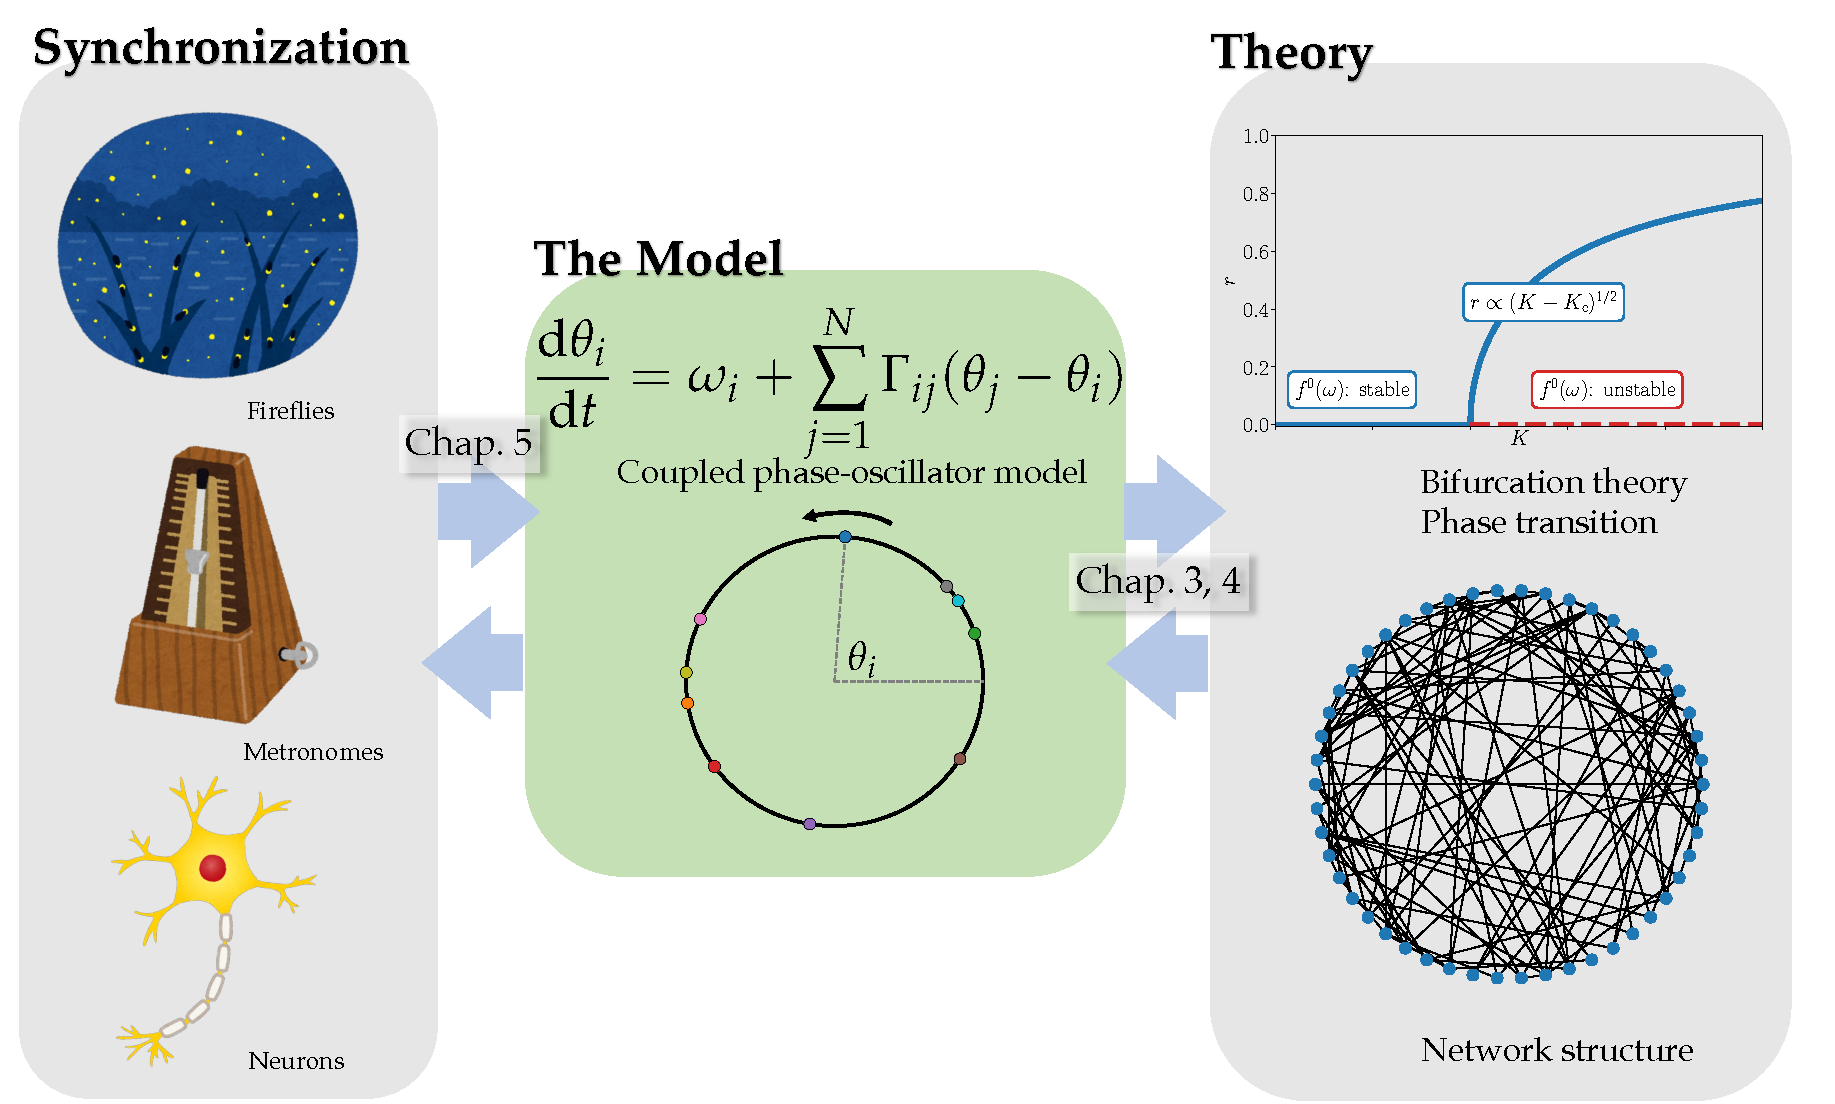
\includegraphics[width=\textwidth]{figs/phd_schematic.pdf}
  \caption{Schematic representation on our study.}
  \label{fig:ponchi}
\end{figure}

\section{Thesis Outline}

We conclude this chapter with an outline of this thesis.

In Chapter~\ref{chap:rev_cpo}, we give a brief review of coupled phase-oscillator models.
Using the Kuramoto model, a representative example of a coupled phase oscillator system, we will review our past research on the conditions for synchronization and the transition phenomena from an asynchronous state to a synchronous state. The critical exponents obtained near the transition point when this transition phenomenon is regarded as a critical phenomenon in statistical mechanics will also be summarized.

Chapter~\ref{chap:paper02} is constructed based on our paper \cite{yoneda2020} entitled ``Critical exponents in coupled phase-oscillator models on small-world networks''.
As in the previous chapter, the synchronization transition is characterized by several critical exponents, and we focus on the critical exponent defined by coupling strength dependence of the order parameter for revealing universality classes. In a typical interaction represented by the perfect graph, an infinite number of universality classes is yielded by dependency on the natural frequency distribution and the coupling function. Since the synchronization transition is also observed in a model on a small-world network, whose number of links is proportional to the number of oscillators, a natural question is whether the infinite number of universality classes remains in small-world networks irrespective of the order of links. Our numerical results suggest that the number of universality classes is reduced to one and the critical exponent is shared in the considered models having coupling functions up to second harmonics with unimodal and symmetric natural frequency distributions.

Chapter~\ref{chap:paper03} is constructed based on our paper \cite{yoneda2021} entitled ``The lower bound of the network connectivity guaranteeing in-phase synchronization''.
In-phase synchronization is a stable state of identical Kuramoto oscillators coupled on a network with identical positive connections, regardless of network topology. However, this fact does not mean that the networks always synchronize in-phase because other attractors besides the stable state may exist. The critical connectivity $\mu_{\mathrm{c}}$ is defined as the network connectivity above which only the in-phase state is stable for all the networks. In other words, below $\mu_{\mathrm{c}}$, one can find at least one network that has a stable state besides the in-phase sync. The best known evaluation of the value so far is $0.6828\dots\leq\mu_{\mathrm{c}}\leq0.7889\dots$. In this paper, focusing on the twisted states of the circulant networks, we provide a method to systematically analyze the linear stability of all possible twisted states on all possible circulant networks. This method using integer programming enables us to find the densest circulant network having a stable twisted state besides the in-phase sync, which breaks a record of the lower bound of the $\mu_{\mathrm{c}}$ from $0.6828\dots$ to $0.6838\dots$. We confirm the validity of the theory by numerical simulations of the networks not converging to the in-phase state.

Chapter~\ref{chap:paper06} is constructed based on our paper \cite{yoneda2022} entitled ``Gaussian process regression approach to estimating phase dynamics from rhythmic data''.
The problem of estimating from data the mathematical model behind natural phenomena has long been studied. Since it has been theoretically shown that rhythmic phenomena, including synchronous phenomena, can be modeled by coupled phase-oscillator models, methods have been proposed to estimate models from real data that show these phenomena. A method in which the coupling function is approximated by a Fourier series expansion of finite order and the Fourier coefficients are estimated by Bayesian linear regression has been used so far, but problems of order determination and the Gibbs phenomenon have sometimes been encountered. In this study, we propose a method to estimate the coupling function using Gaussian process regression. By setting the covariance function to a periodic kernel, we expect to estimate a smooth periodic function. We report the successful application of Gaussian process regression to a network model of van der Pol oscillators and spiking neurons to accurately estimate the coupling function.

Finally we conclude this thesis in Chapter~\ref{chap:conclusion} and discuss some future works.
% We also give a brief review on Gaussian process regression in Appendix~\ref{chap:gp}, which is a statistical method used to derivating the coupled phase-oscillator model from given data in Chapter~\ref{chap:paper06}.
